\chapter{Grundlagen}
\label{ch:Grundlagen}


UDP

Beim User Datagram Protocol handelt es sich um ein verbindungsloses und in jeglicher Hinsicht ungeschütztes Protokoll, das auf der Transportebene (Schicht 4 im OSI-Schichtenmodell) arbeitet. Es bestehen keinerlei Mechanismen, die das korrekte Übertragen von Paketen gewährleisten. Hierzu zählen:

\begin{description}
	\item[Sicherheit] Die Sicherheit, dass Pakete überhaupt ankommen
	\item[Reihenfolge] Die Reihenfolge, in der Pakete ankommen
	\item[FlowControl] Ein Überlaufschutz des Empfängerspeichers (FlowControl)
	\item[CongestionControl] Stauvermeidung in der Übertragungskette (CongestionControl)
	\item[Angriffe] Schutz gegen Paketmanipulation von dritten
\end{description}

\begin{figure}
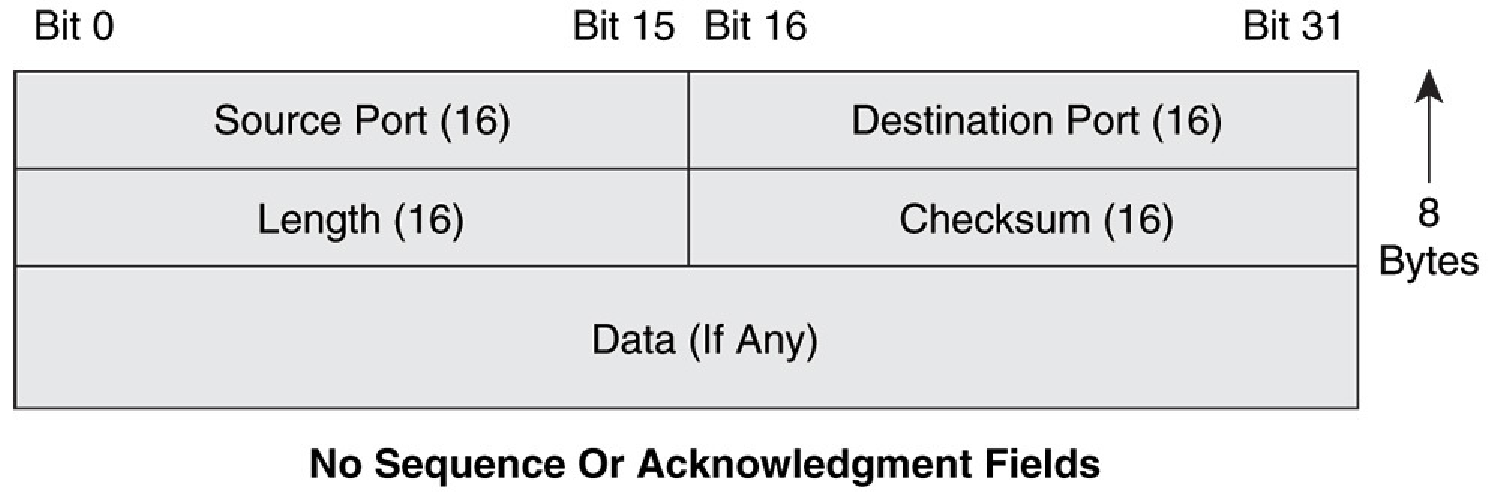
\includegraphics[width=\textwidth]{images/UDP_header.pdf}
\caption{UDP Header}
\label{fig:udp_header}
\end{figure}

Ein UDP Header besteht aus 8 Byte. Mit diesen 8 Byte werden lediglich Source-Port, Destination-Port, Länge und die Checksumme übertragen. Dieser vergleichsweise kleine Header (vgl. TCP mit etwa 20 Byte), führt zu einem geringen Overhead während der Übertragung, auch bei kleinen Paketen. Nachdem ein Paket gesendet wurde erfolgt keine Bestätigung des Pakets vom Empfänger. Durch diesen Uni-Direktionalen Sendevorgang entsteht wenig Traffic im Netzwerk. Falls gewisse Sicherheitsmechanismen gewünscht sind, müssen diese in höheren Schichten implementiert werden. \\
Aufgrund dieser Eigenschaften wird UDP in Bereichen eingesetzt, in denen es auf hohe Übertragungsgeschwindigkeit ankommt und eventuelle Paketverluste zu verkraften sind, bzw. von höheren Schichten aufgelöst werden.




\newpage


TCP

Beim Transmission Control Protocol handelt es sich um ein verbindungsorientiertes paketvermittelndes Protokoll. Mithilfe verschiedener Mechanismen wird sichergestellt, dass Pakete in der richtigen Reihenfolge ankommen, es zu keinen Staus kommt und dass Netzwerkknoten nicht überlaufen. Dadurch, dass das Protokoll verbindungsorientiert arbeitet, können beide Teilnehmer der Verbindung Daten ohne Anfragen senden. 

\begin{figure}
	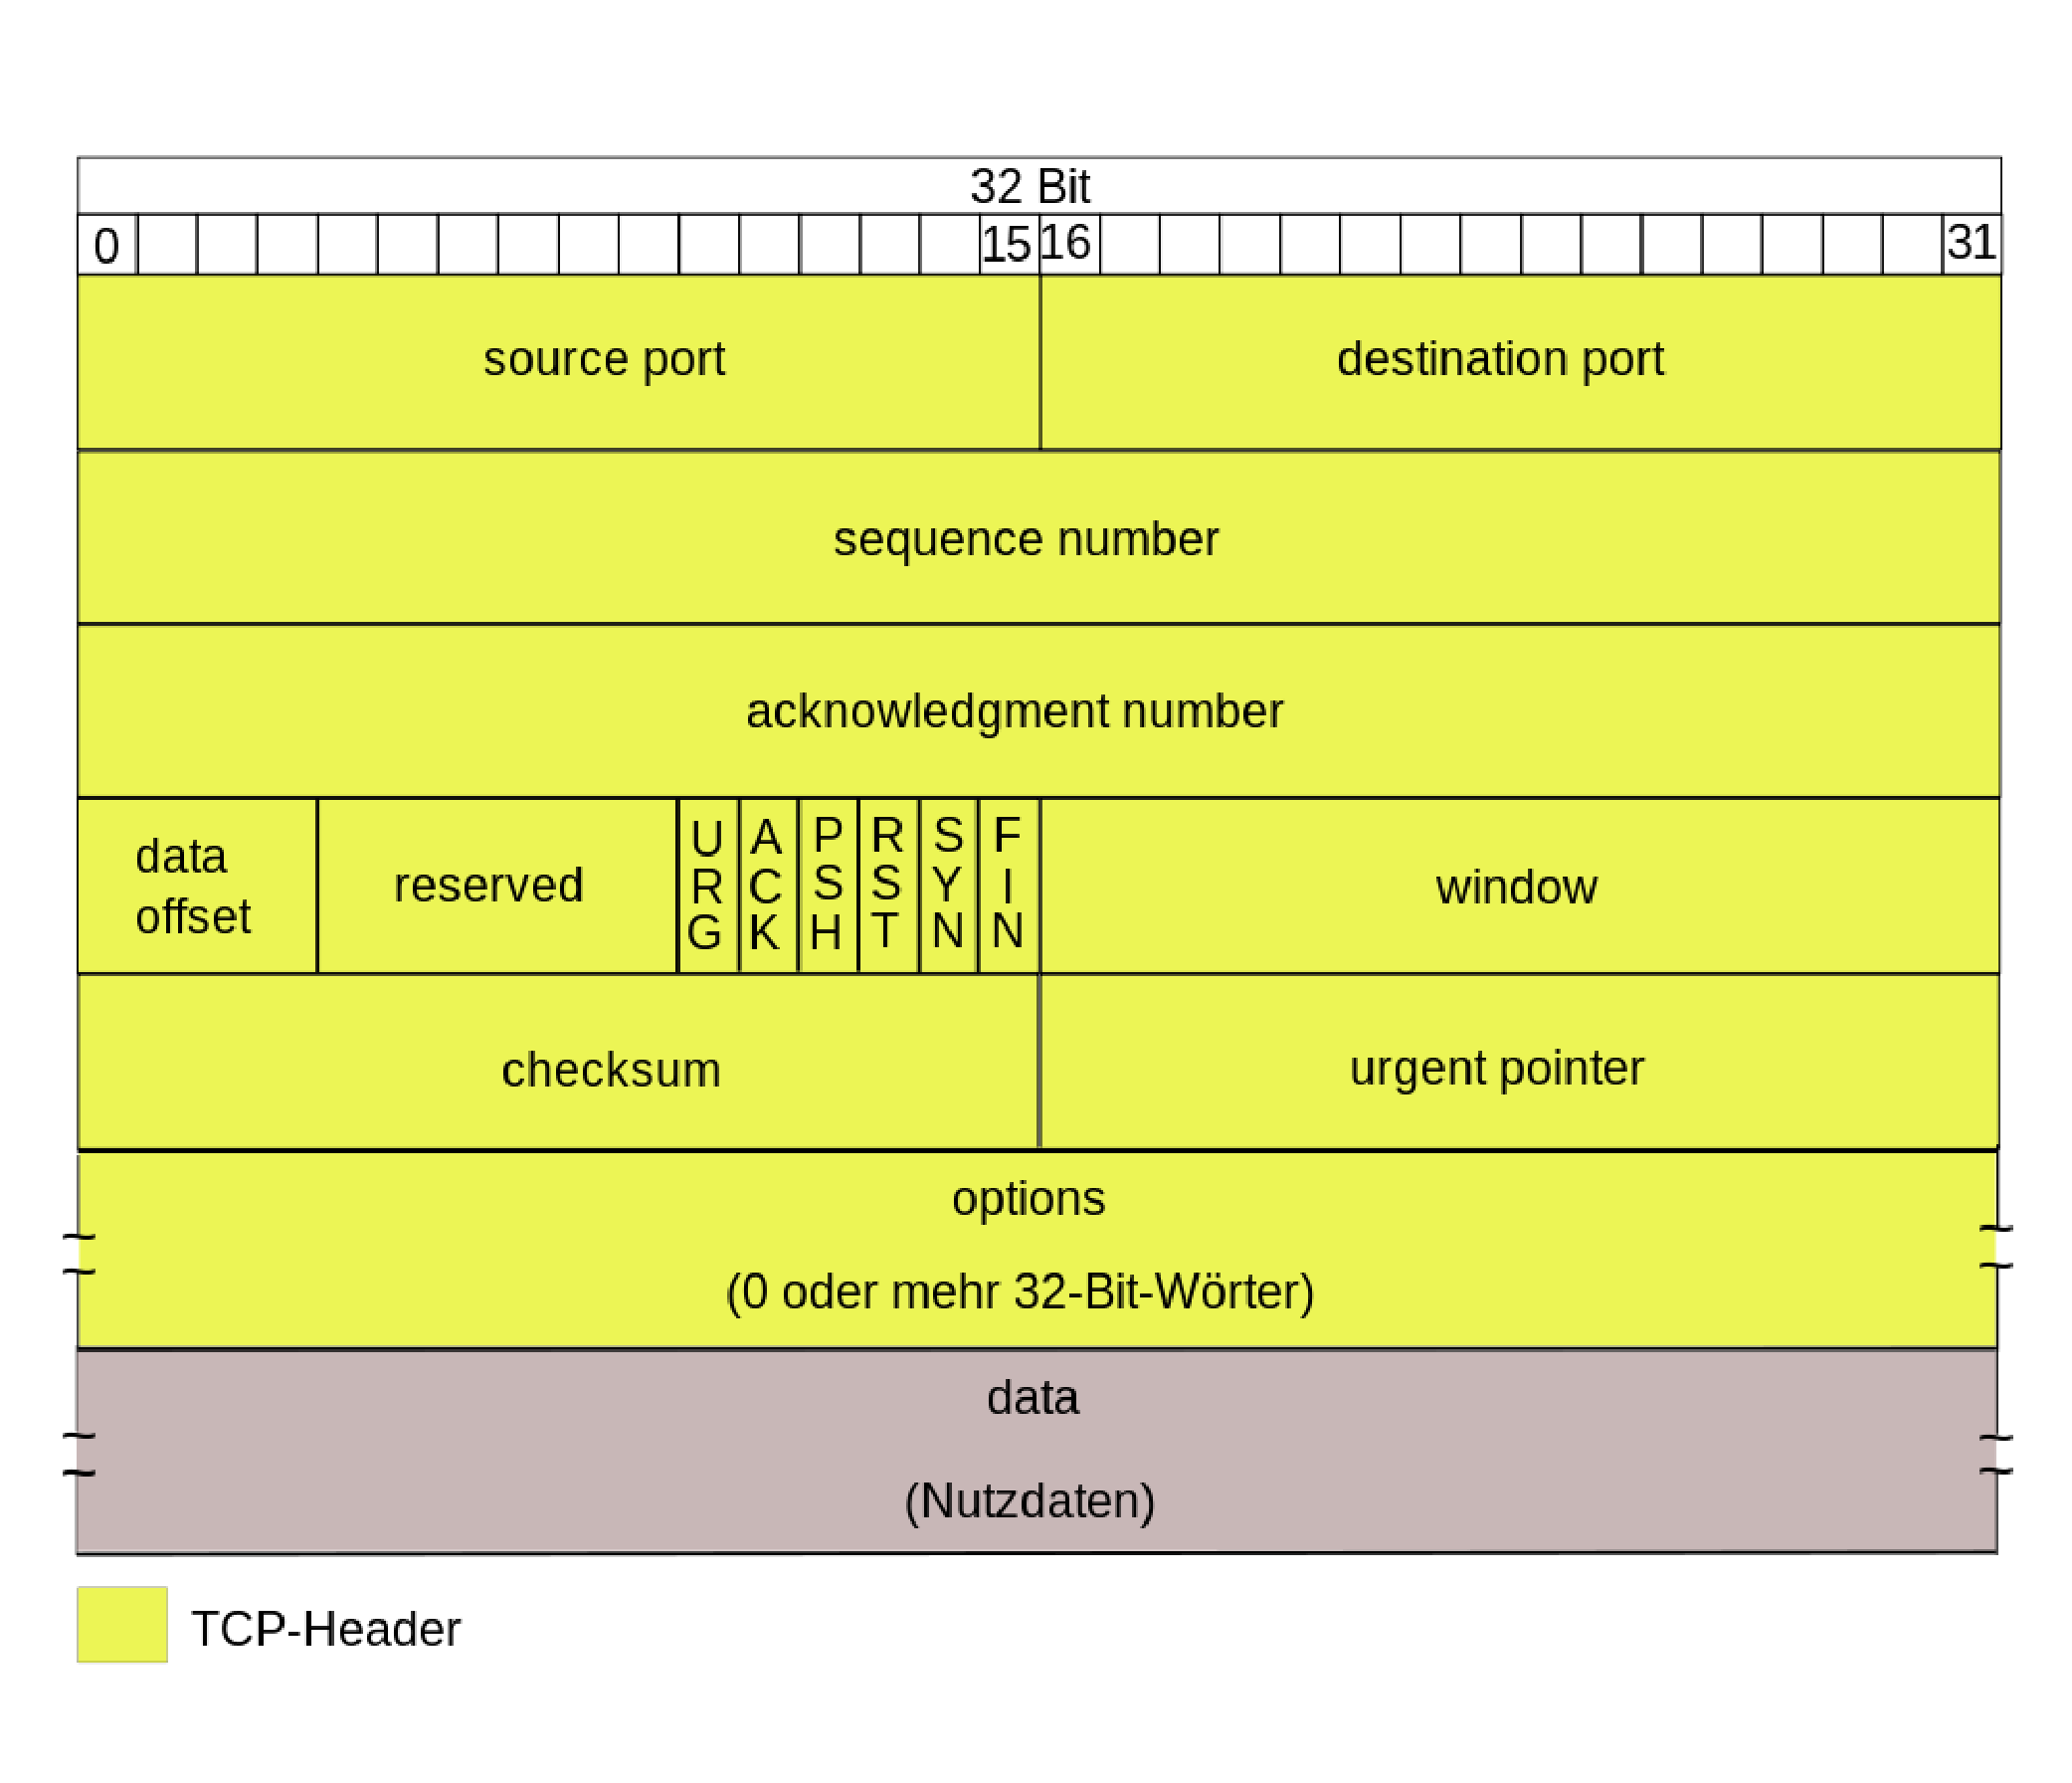
\includegraphics[width=\textwidth]{images/TCP_header.pdf}
	\caption{TCP Header}
	\label{fig:tcp_header}
\end{figure}

Durch den größeren Header und dem größeren Traffic, der das Protokoll verursacht, wird TCP für Anwendungen verwendet, bei denen ein Paketverlust ausgeschlossen werden soll, dafür aber eine etwas höhere Latenz in Kauf genommen werden kann. 
Die Verbindung wird über einen 3-Wege-Handshake hergestellt. Hierbei sendet ein Teilnehmer eine Anfrage (syn), diese wird bestätigt (syn ack) woraufhin die Bestätigung erneut bestätigt wird. In diesem dritten Schritt werden meist bereits die ersten Nutzdaten mitgesendet.
\begin{figure}
	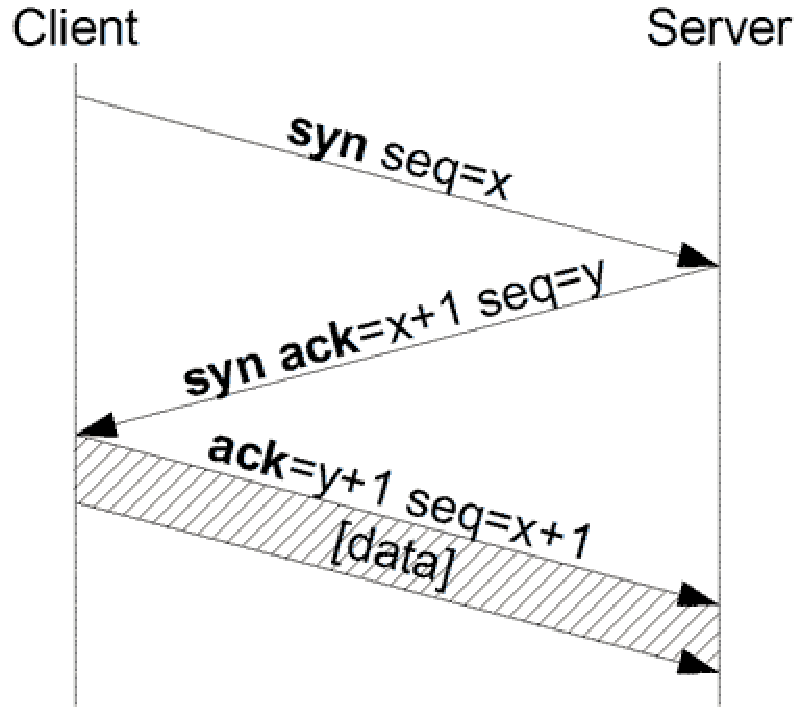
\includegraphics[width=\textwidth]{images/TCP_3wayhandshake.pdf}
	\caption{TCP 3-Wege-Handshake}
	\label{fig:tcp_3wayhandshake}
\end{figure}

Mithilfe von geordneten Sequenznummern und Acknowledgments werden alle empfangene Pakete bestätigt. Durch das Fehlen einer Sequenznummer erkennt der Empfänger den Verlust eines Pakets und teilt daraufhin dem Sender mit, dass es nicht angekommen ist. Für den Fall eines Verlusts des Acknowledgments, hat der Sender einen Timer, welcher nach einiger Zeit eine Retransmission des Pakets veranlasst, sofern kein Acknowledgment ankommen sollte.

Flow-Control:



Congestion-Control